\documentclass[12pt, a4paper]{article}

\usepackage{graphicx}
\graphicspath{ {./images/} }
%Tarih Ekleme
\usepackage[ddmmyyyy]{datetime}
\renewcommand{\dateseparator}{.}
\renewcommand{\figurename}{Şekil}
\renewcommand{\refname}{Kaynakça}

% Başlık stili
\usepackage{titling}
\pretitle{\begin{center}\LARGE\bfseries}
	\posttitle{\end{center}}

%Hafta1

\title{Artırılmış Gerçeklik Ansiklopedisi Raporu Hafta 1 }
\author{Hasan Tekin}
\date{\today}
%\date{\DTMnow}
%\date{\DTMnow}


\begin{document}
	\maketitle
	
	
	
	\section{Proje Amacı}
	Bu projenin amacı, Vuforia ve Unity kullanarak bir artırılmış gerçeklik ansiklopedisi oluşturmak ve kullanıcılara gerçek dünya nesneleri ile etkileşimli bir şekilde bilgi sunmaktır. Ansiklopedi içeriği,3D modeller, metinler ve görsellerden oluşmaktadır.
	\section{Vuforia Nedir ?}
	
	Vuforia, artırılmış gerçeklik (AR) deneyimleri geliştirmek için kullanılan bir platformdur. Geliştiricilere, mobil cihazlar, tabletler ve akıllı gözlükler gibi cihazlarda çalışan interaktif AR uygulamaları oluşturma imkanı sağlar.
	
	Vuforia, birçok farklı endüstride kullanılabilecek geniş bir özellik yelpazesine sahiptir. Ürün tanıtımından eğitim ve eğlenceye kadar birçok farklı alan için kullanılabilir. Örneğin, Vuforia ile bir şirket ürününü interaktif bir şekilde sergileyebilir veya bir eğitim uygulamasında belirli nesnelerin tanımlanmasını sağlayabilirsiniz.
	
	Bu platform, görüntü tanıma, nesne tanıma, işaretleme ve bulut tabanlı hizmetler gibi çeşitli AR teknolojilerini destekler.Vuforia, Unity ve diğer popüler oyun motorlarıyla entegre olabilen bir geliştirme platformudur, bu da geliştiricilerin AR deneyimlerini oluşturmak için geniş bir araç yelpazesinden yararlanmalarını sağlar.\cite{Vuforia}
	
	
	\section{Vuforia Nasıl Kullanılır ?}
	
	\newpage
	\begin{figure}[!ht]
		\caption{}
		\centering
		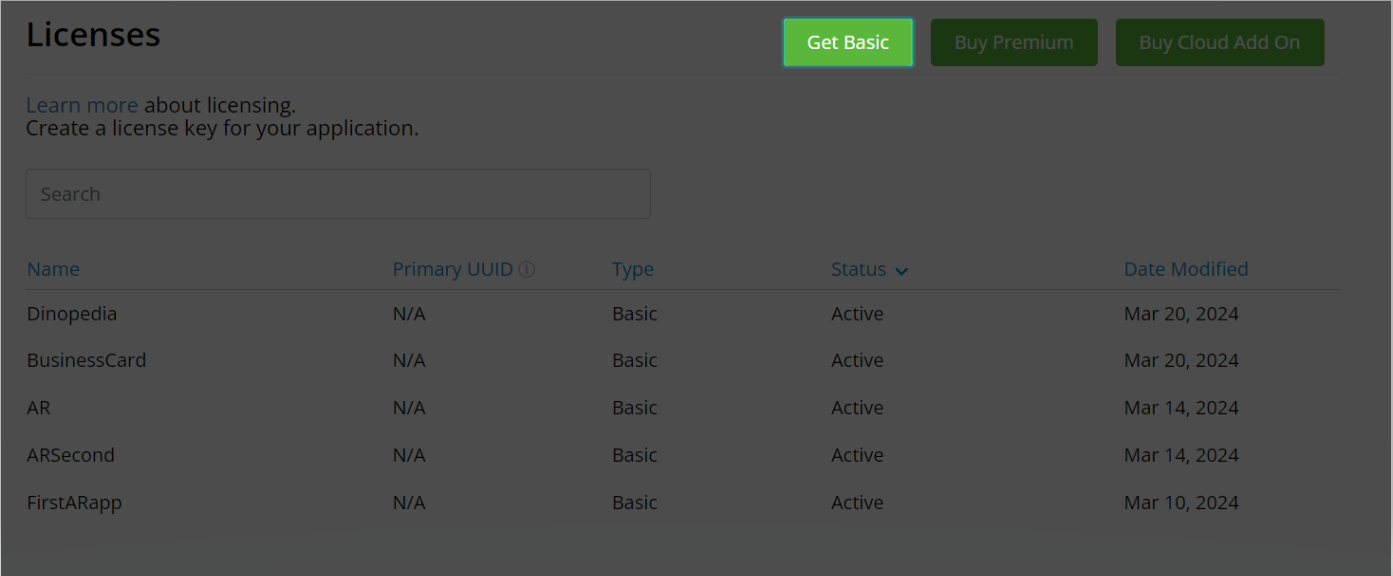
\includegraphics[angle=0, width=\textwidth]{Vuforia2.PNG}
		\label{gantt}
		Şekil \ref{gantt} de lisans sayfası gösterilmiştir.\cite{Vuforia}	
		
		
		
	\end{figure}
	
	\begin{figure}[!ht]
		\caption{}
		\centering
		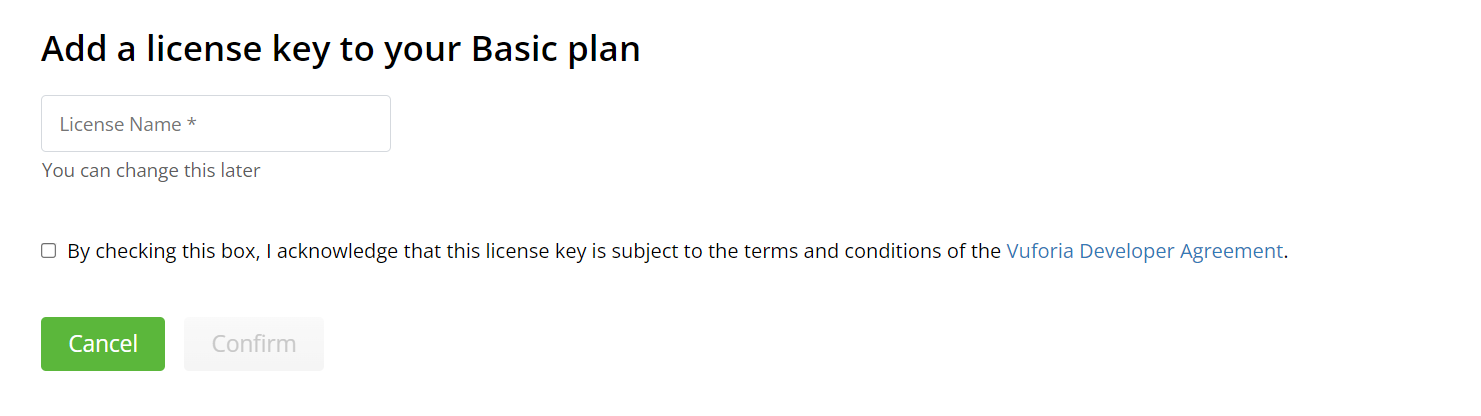
\includegraphics[angle=0, width=\textwidth]{Vuforia3.PNG}
		
		\label{gantt1}
		Şekil \ref{gantt1} de lisans sayfasında yeni bir lisans oluşturmanın ilk adımı gösterilmiştir.\cite{Vuforia}	
		
		
	\end{figure}
	\newpage
	\begin{figure}[!ht]
		\caption{}
		\centering
		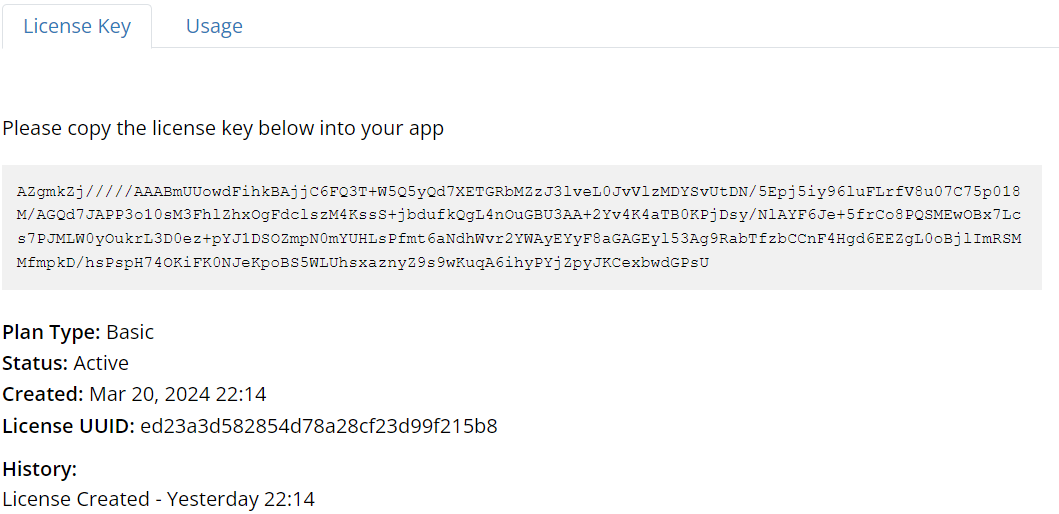
\includegraphics[angle=0, width=\textwidth]{Vuforia4.PNG}
		
		\label{gantt2}
		Şekil \ref{gantt2} de oluşturulan lisans gösterilmiştir.\cite{Vuforia}	
	\end{figure}
	
	\begin{figure}[!ht]
		\caption{}
		\centering
		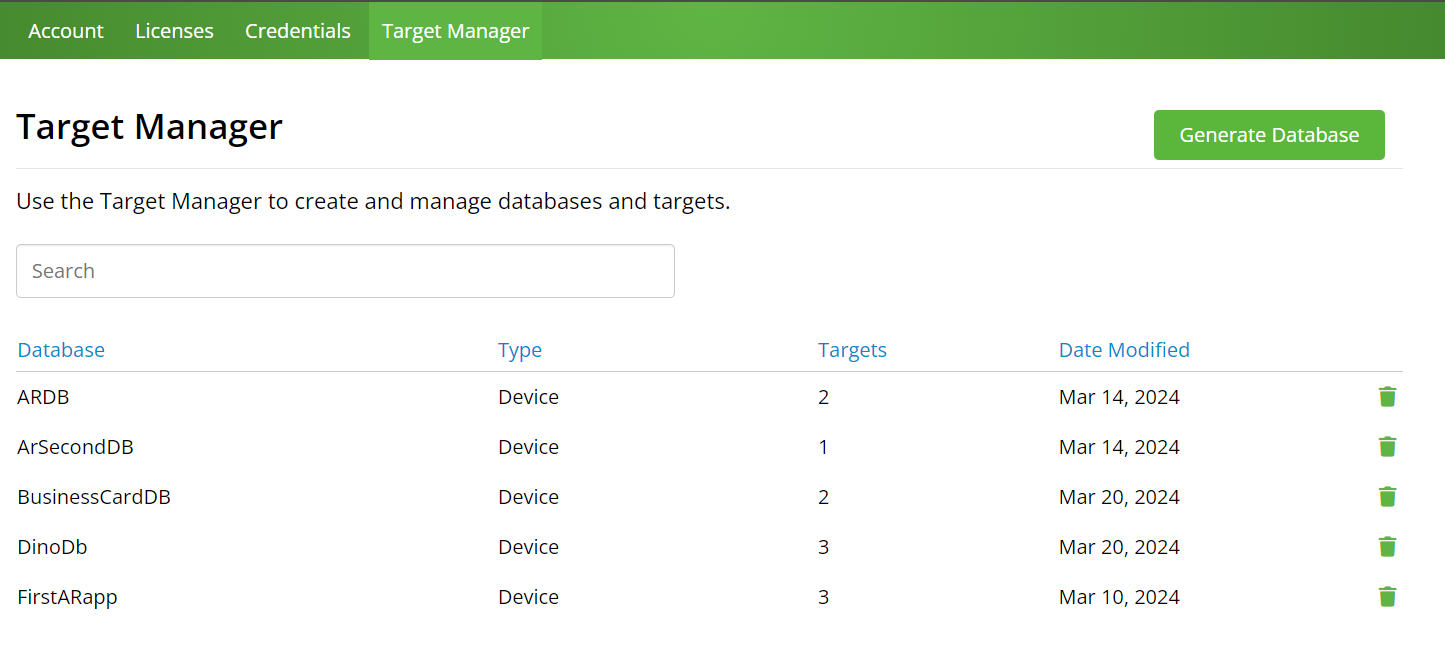
\includegraphics[angle=0, width=\textwidth]{Vuforia5.PNG}
		
		\label{gantt3}
		Şekil \ref{gantt3} de Target Manager için database oluşturma penceresi gösterilmiştir.\cite{Vuforia}	
	\end{figure}
	\newpage
	\begin{figure}[!ht]
		\caption{}
		\centering
		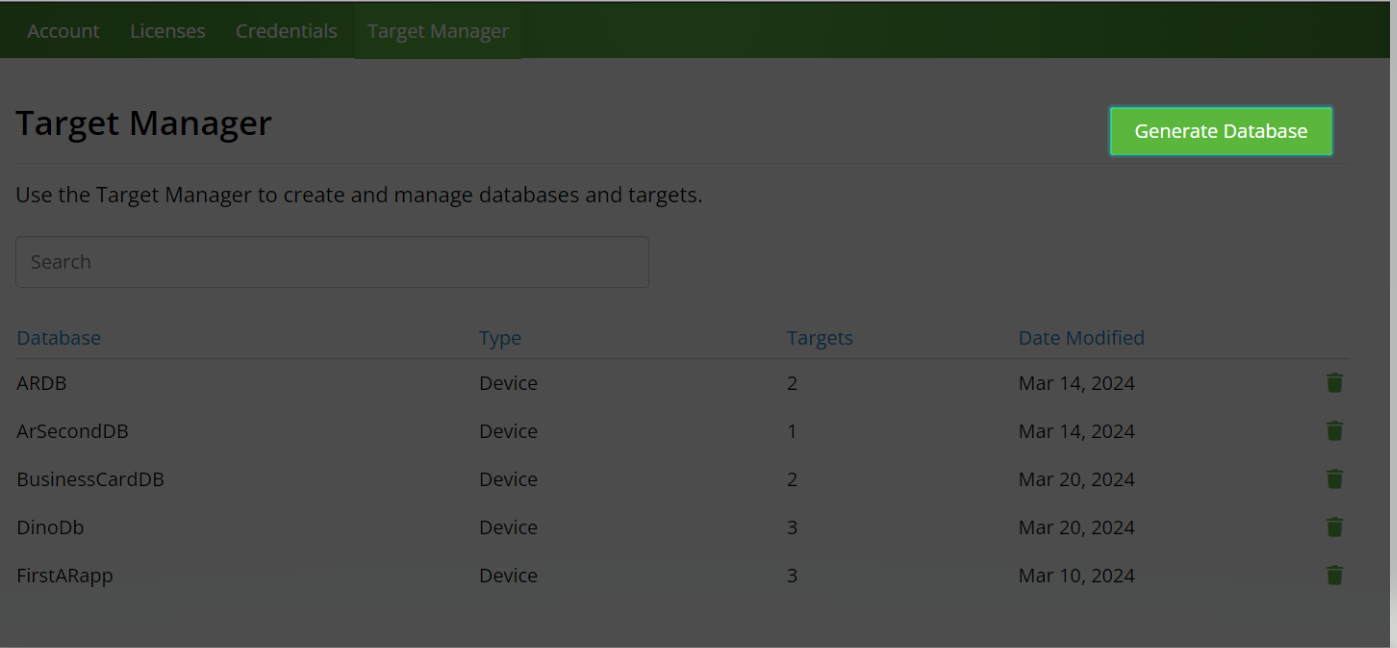
\includegraphics[angle=0, width=\textwidth]{Vuforia6.PNG}
		
		\label{gantt4}
		Şekil \ref{gantt4} de Target Manager için database oluşturmanın ilk adımı gösterilmiştir.\cite{Vuforia}	
	\end{figure}
	\begin{figure}[!ht]
		\caption{}
		\centering
		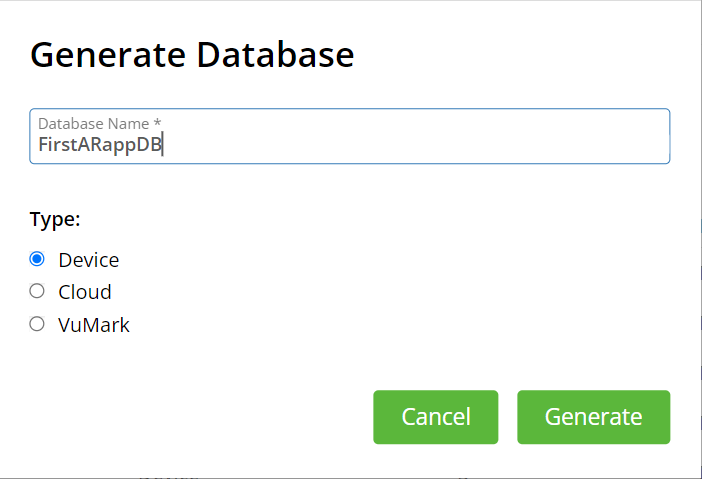
\includegraphics[angle=0, width=\textwidth]{Vuforia7.PNG}
		
		\label{gantt5}
		Şekil \ref{gantt5} de  database ismini verdiğimiz pencere gösterilmiştir.\cite{Vuforia}	
	\end{figure}
	\begin{figure}[!ht]
		\caption{}
		\centering
		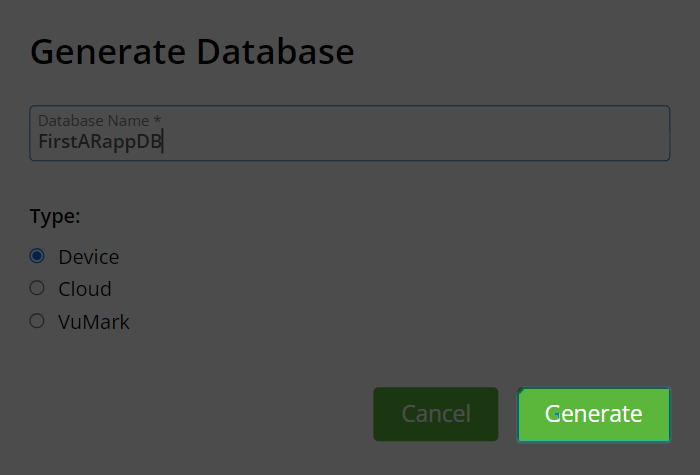
\includegraphics[angle=0, width=\textwidth]{Vuforia8.PNG}
		
		\label{gantt6}
		Şekil \ref{gantt6} de  database ismini verdikten sonra yapılacak işlem gösterilmiştir.\cite{Vuforia}	
	\end{figure}
	\newpage
	\begin{figure}[!ht]
		\caption{}
		\centering
		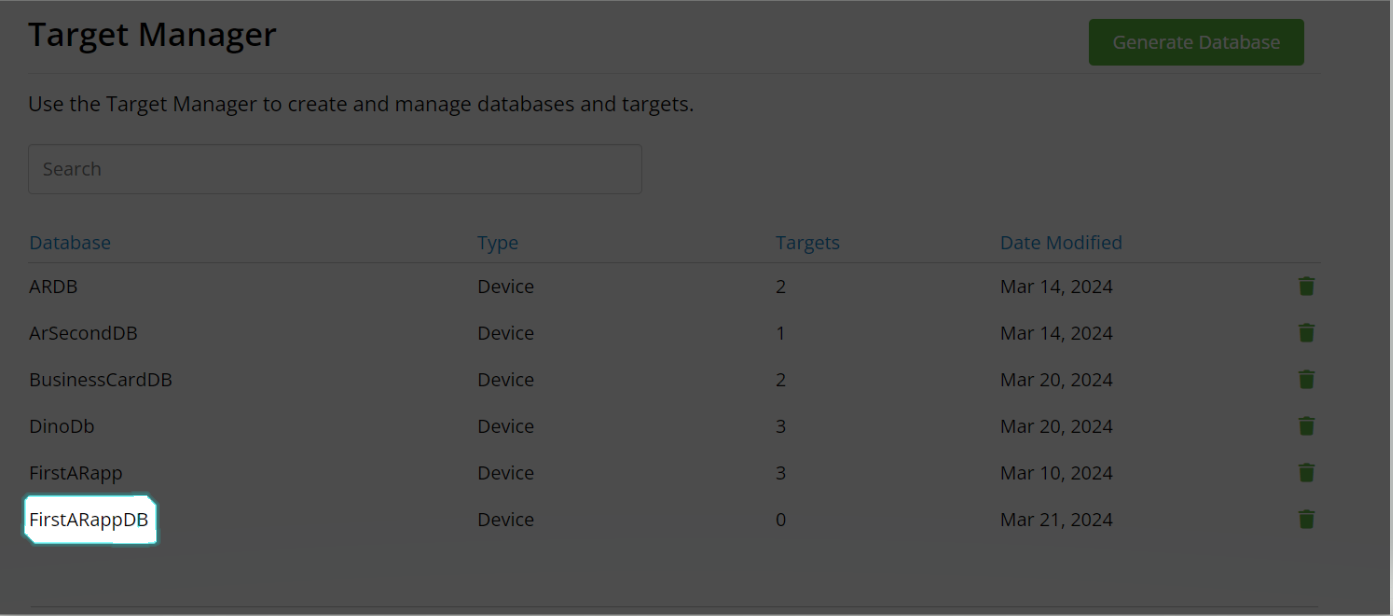
\includegraphics[angle=0, width=\textwidth]{Vuforia9.PNG}
		
		\label{gantt7}
		Şekil \ref{gantt7} de oluşturduğumuz databese gösterilmiştir.\cite{Vuforia}	
	\end{figure}
	\newpage
	\begin{figure}[!ht]
		\caption{}
		\centering
		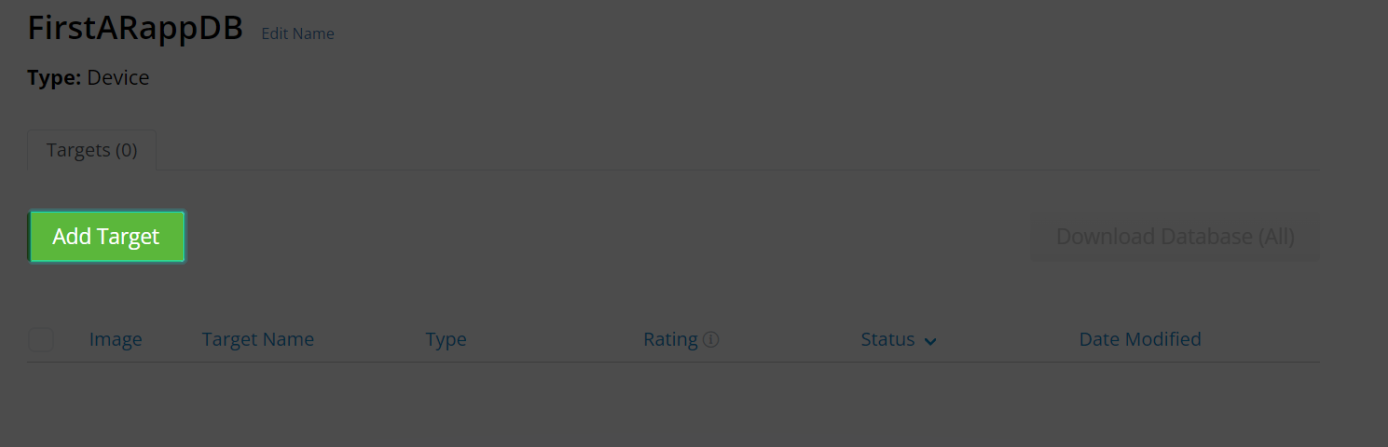
\includegraphics[angle=0, width=\textwidth]{Vuforia10.PNG}
		
		\label{gantt8}
		Şekil \ref{gantt8} de target eklemek istediğimizde kullanılacak kısım gösterilmiştir.\cite{Vuforia}	
	\end{figure}
	\newpage
	\begin{figure}[!ht]
		\caption{}
		\centering
		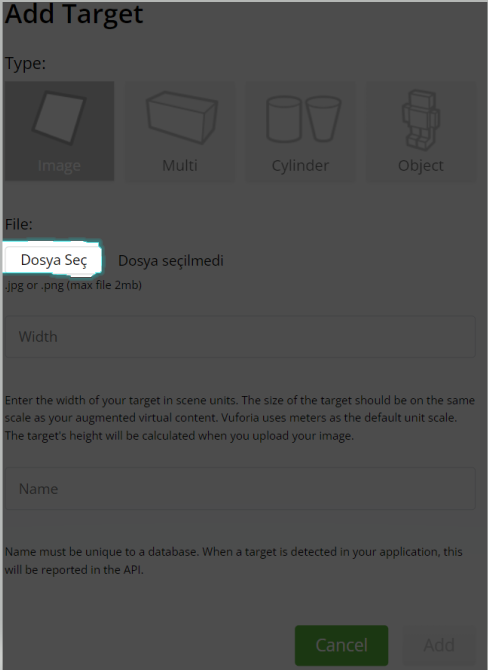
\includegraphics[angle=0, width=\textwidth]{Vuforia12.PNG}
		
		\label{gantt9}
		Şekil \ref{gantt9} de eklemek istediğimiz target seçme işlemi gösterilmiştir.\cite{Vuforia}	
	\end{figure}
	\begin{figure}[!ht]
		\caption{}
		\centering
		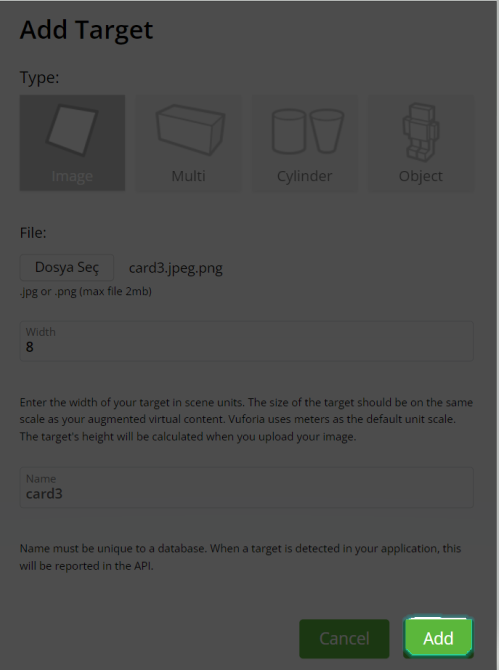
\includegraphics[angle=0, width=\textwidth]{Vuforia13.PNG}
		
		\label{gantt10}
		Şekil \ref{gantt10} de target eklemenin son adımı gösterilmiştir.\cite{Vuforia}
	\end{figure}
	\begin{figure}[!ht]
		\caption{}
		\centering
		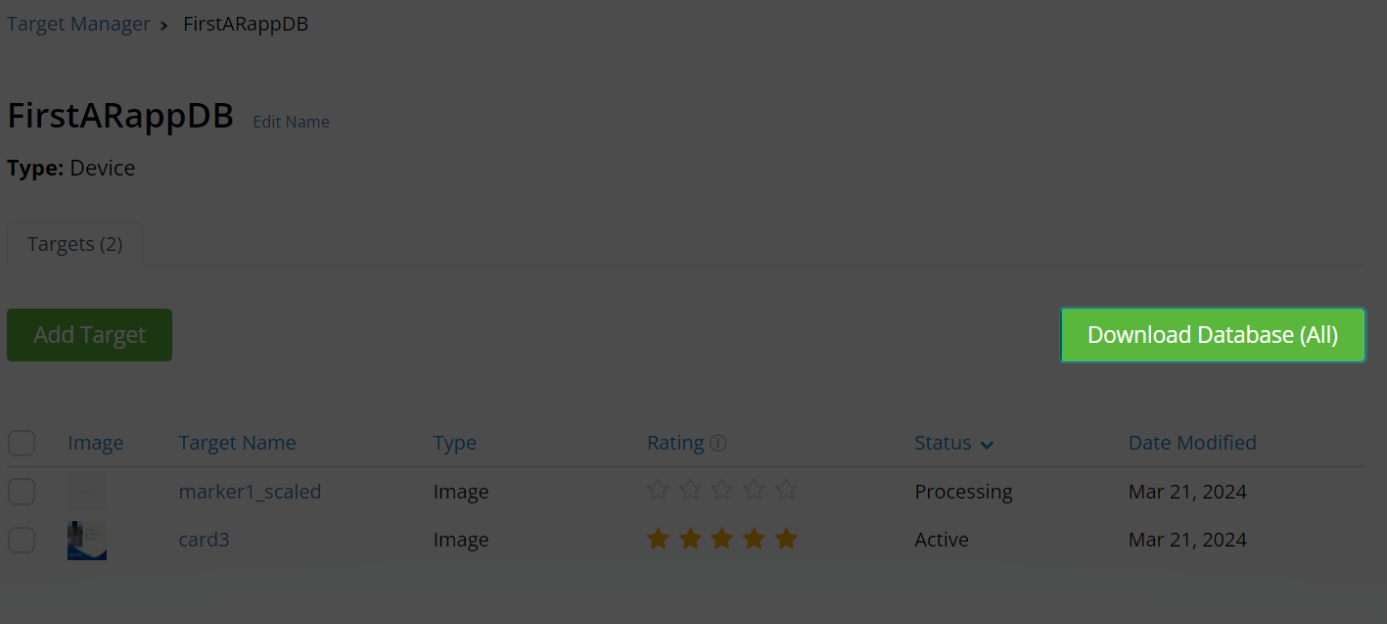
\includegraphics[angle=0, width=\textwidth]{Vuforia14.PNG}
		
		\label{gantt11}
		Şekil \ref{gantt11} de oluşturduğumuz target indirmek için ilk adım gösterilmiştir.\cite{Vuforia}
	\end{figure}
	\newpage
	\begin{figure}[!ht]
		\caption{}
		\centering
		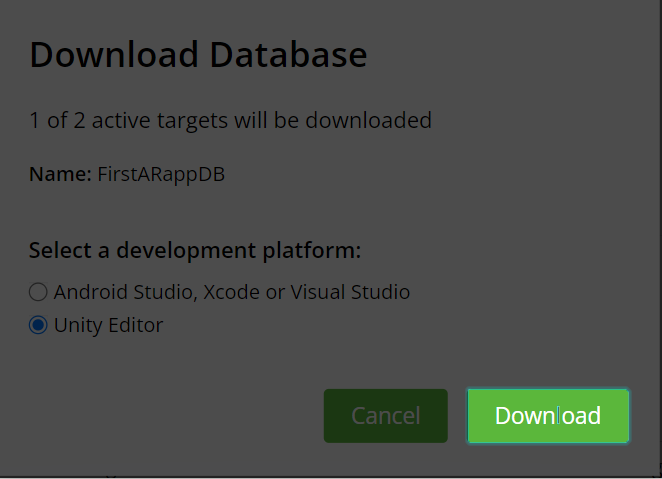
\includegraphics[angle=0, width=\textwidth]{Vuforia15.PNG}
		
		\label{gantt12}
		Şekil \ref{gantt12} de oluşturduğumuz target indirmek için son adım gösterilmiştir.\cite{Vuforia}
	\end{figure}
	\setcounter{section}{0}
	\newpage
		\title{Artırılmış Gerçeklik Ansiklopedisi Raporu Hafta 2}
	\author{}
	\date{}
	\maketitle
	
	\section{Amaç}
	\begin{enumerate}
		\item Artırılmış Gerçeklik Ansiklopedisi uygulaması, kullanıcılara dünyada çok uzun zaman önce yaşamış  dinazorlar hakkında 3D modeller ve metinlerle bilgi sunmayı amaçlar.\cite{Encyclopedia}
	\end{enumerate}
	
	\section{Uygulamanın Özellikleri}
	\begin{enumerate}
		\item Geniş Kapsamlı İçerik: Uygulama, kullanıcıların dinazorlar hakkında bilgi edinebilmeleri sağlayan içeriğe sahiptir.
		\item   3D Modeller ve Görseller: Ansiklopedi içeriği,3D modeller ve görseller kullanılarak zenginleştirilmiştir.
		Metinler ve Açıklamalar: Kullanıcılar, dinazorlar hakkında detaylı metinler ve açıklamaları okuyabilirler.\cite{GitHub}
		
	\end{enumerate}
	
	
	
	
	\section{Kullanılan Teknolojiler}
	\begin{enumerate}
		\item Teknoloji Kullanımı:
		Vuforia ve Unity Entegrasyonu: Uygulama, Vuforia ve Unity gibi artırılmış gerçeklik platformlarını kullanarak nesneleri tanır ve içerikleri görüntüler.
		
	\end{enumerate}
	\newpage
	\begin{figure}[!ht]
		\caption{}
		\centering
		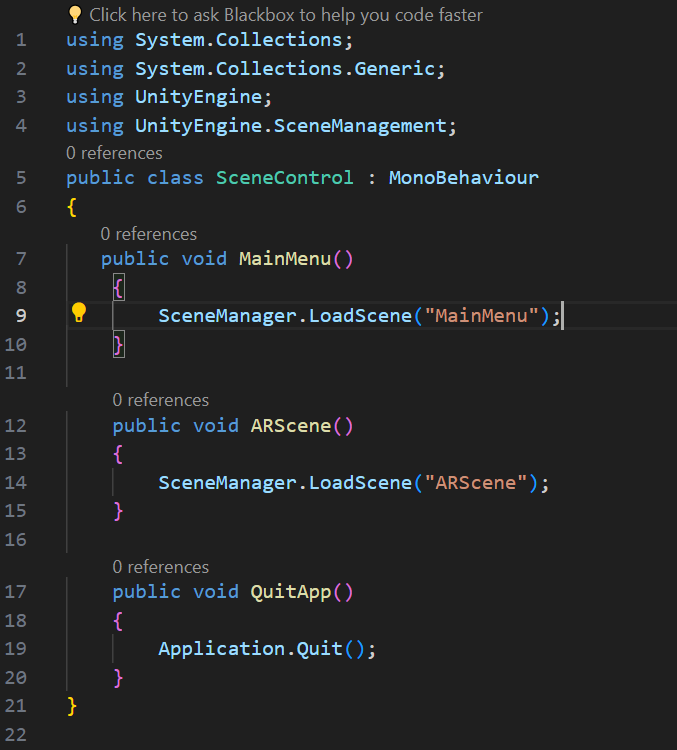
\includegraphics[width=0.8\textwidth]{dinoAR.PNG}
		
		\label{dinoo}
	\end{figure}
	Şekil \ref{dinoo} de gösterildiği gibi bu kod Unity uygulamalarında kullanıcı arayüzü üzerinde butonlara bağlanarak farklı sahneler arasında geçiş yapmak veya uygulamayı kapatmak için kullanılır.\cite{GitHub}
	\newpage
	\begin{figure}[!ht]
		\caption{}
		\centering
		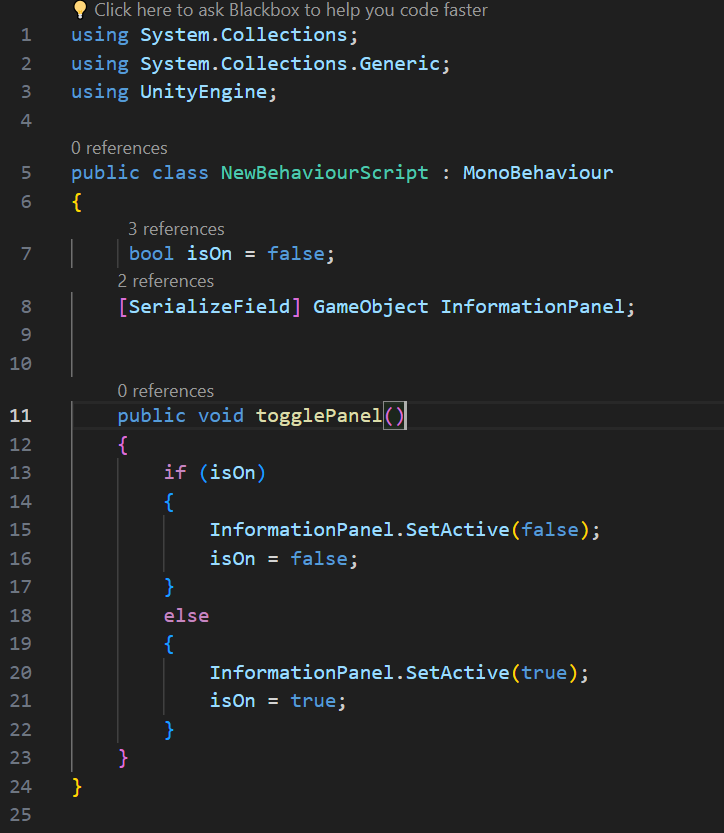
\includegraphics[width=0.8\textwidth]{dinoAR2.PNG}
		
		\label{dino2}
	\end{figure}
	Şekil \ref{dino2} deki bu kod, basit bir toggle mantığı kullanarak bir panelin açık veya kapalı olup olmadığını kontrol eder. Eğer panel açıksa, düğmeye tıklandığında kapanır; kapalıysa, tıklandığında açılır.\cite{GitHub}
	
	\title{Artırılmış Gerçeklikle Mobilya Görüntüleme Uygulaması Raporu}
	\author{}
	\date{}
	\maketitle
	% Section değerini sıfırlıyor alt başlık değerini
	\setcounter{section}{0}
	
	\section{Amaç}
	\begin{enumerate}
		\item Furniture AR uygulaması, kullanıcıların seçtikleri mobilyaları sanal bir ortamda gerçek dünya mekanlarına yerleştirmelerine olanak tanır. Bu uygulama, kullanıcılara mobilya alışverişi yapmadan önce ürünlerin nasıl görüneceğini daha iyi anlamalarına yardımcı olur.\cite{FurnishAR}
	\end{enumerate}
	\section{Uygulamanın Özellikleri}
	\begin{enumerate}
		\item 3D Mobilya Modelleri: Uygulama, kullanıcıların seçtikleri mobilyaları gerçek boyutta ve detaylı bir şekilde görmelerini sağlayan 3D modeller içerir.
		\item  Gerçek Zamanlı Yerleştirme: Kullanıcılar, mobil cihazlarını kullanarak seçtikleri mobilyaları gerçek zamanlı olarak belirledikleri mekanlara yerleştirebilirler.\cite{drive}
		
	\end{enumerate}
	
	
	\section{Kullanılan Teknolojiler}
	\begin{enumerate}
		
		\item	ARCore Entegrasyonu: Uygulama, Google'ın ARCore artırılmış gerçeklik platformunu kullanarak mobil cihazların konumunu ve çevresini algılar.
	\end{enumerate}
	
	\newpage
	\begin{figure}[!ht]
		\caption{}
		\centering
		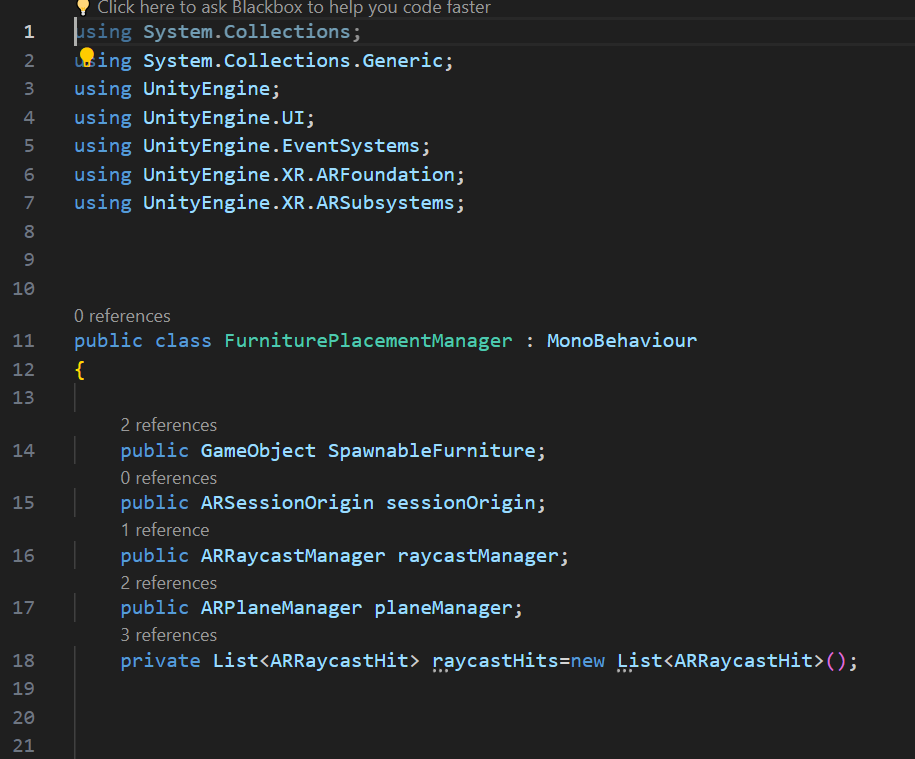
\includegraphics[width=0.8\textwidth]{Ekran.PNG}
		
		\label{mobilya1}
	\end{figure}
	Şekil \ref{mobilya1} deki Bu kod,ilk önce kullanılacak kütüphaneleri çağırır. Ardından  sınıfın üye değişkenlerini tanımlanır. SpawnableFurniture, yerleştirilecek mobilya öğesinin bir referansını alır. sessionOrigin, AR uygulamasında sahnenin orijinalini temsil eder. raycastManager, AR nesnelerinin (örneğin, mobilya öğelerinin) yerleştirileceği gerçek dünya yüzeyini tespit etmek için kullanılır. planeManager, AR'deki düzlemleri yönetmek için kullanılır. raycastHits, raycasting işlemi sırasında elde edilen çarpma bilgilerini saklar.\cite{drive}
	\begin{figure}[!ht]
		\caption{}
		\centering
		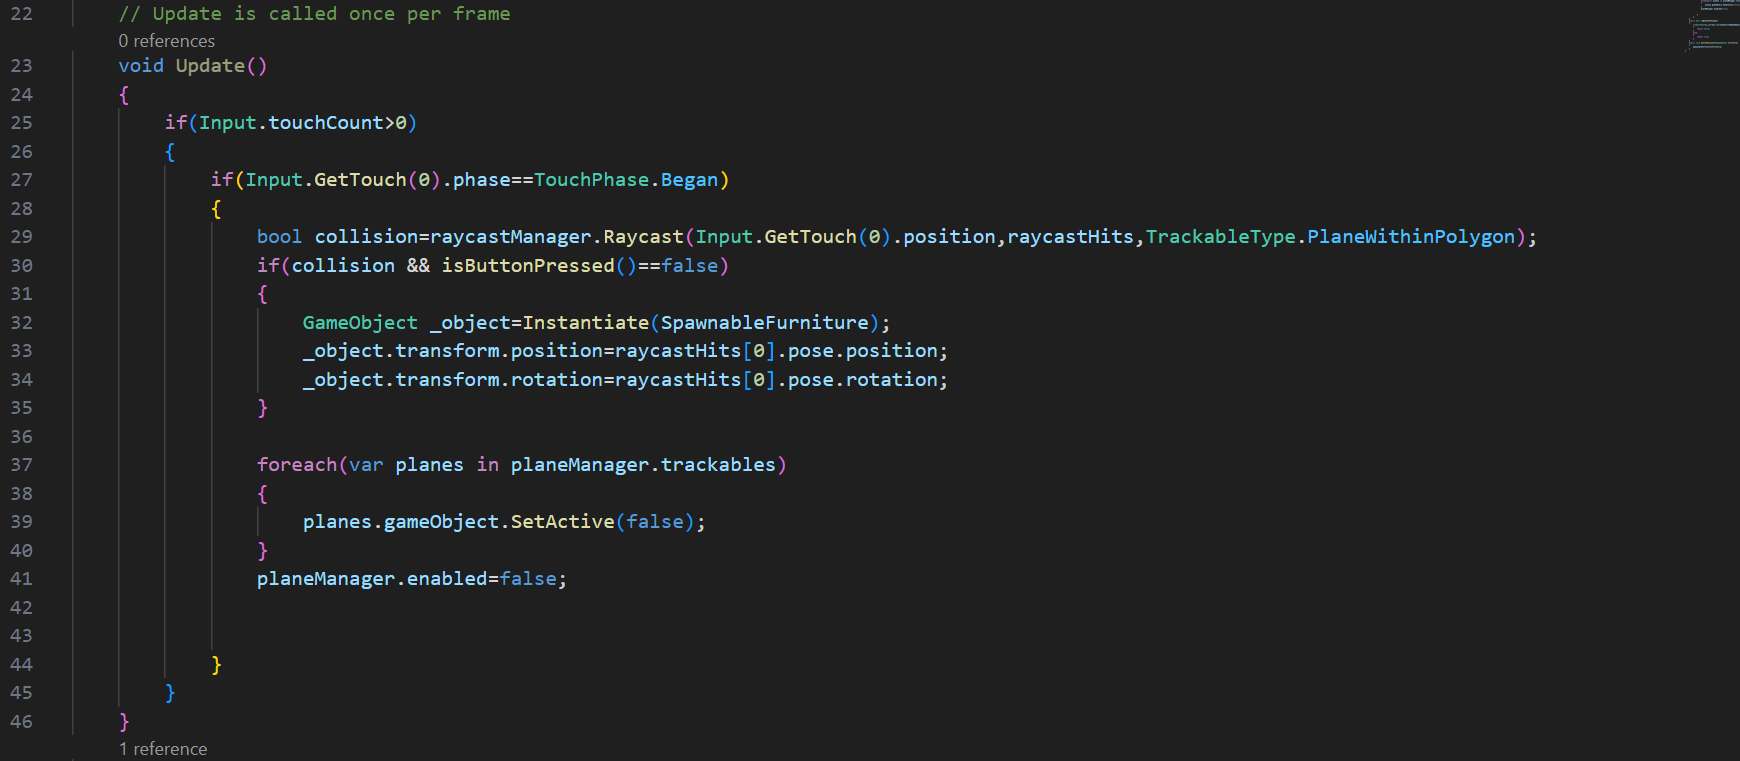
\includegraphics[width=0.8\textwidth]{Ekran2.PNG}
		
		\label{mobilya2}
	\end{figure}
	\newpage
	Şekil \ref{mobilya2} deki bu kodda eğer bir dokunma algılanmışsa ve belirli bir düğme basılmamışsa, mobilyanın yerleştirilmesi için gerekli işlemler gerçekleştirilir.\cite{drive}
	
	\begin{figure}[!ht]
		\caption{}
		\centering
		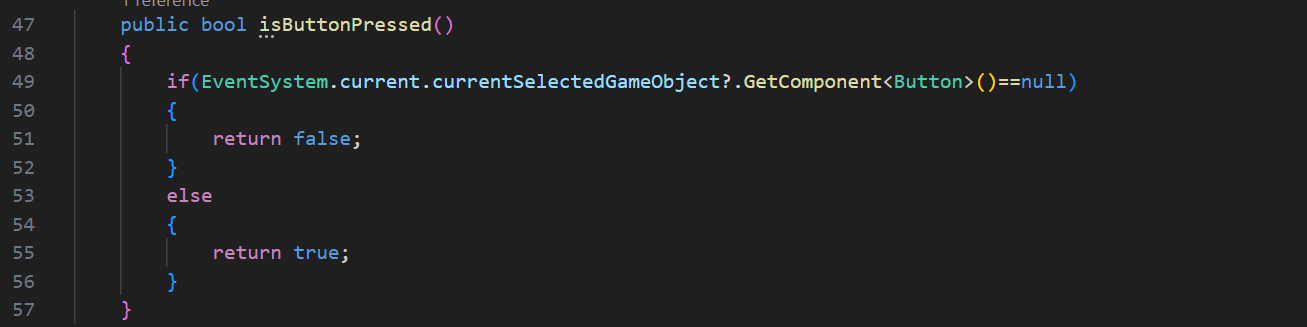
\includegraphics[width=0.8\textwidth]{Ekran4.PNG}
		
		\label{mobilya3}
	\end{figure}
	
	Şekil \ref{mobilya3} deki bu fonksiyon da, kullanıcının herhangi bir butona basıp basmadığını kontrol eder.\cite{drive}
	\begin{figure}[!ht]
		\caption{}
		\centering
		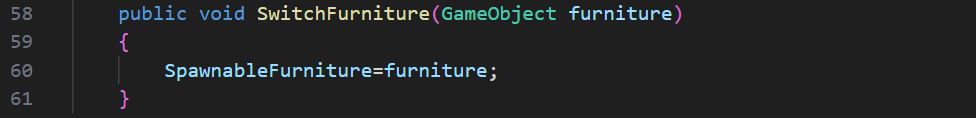
\includegraphics[width=0.8\textwidth]{Ekran5.PNG}
		
		\label{mobilya4}
	\end{figure}
	\newpage
	Şekil \ref{mobilya4} deki bu fonksiyon da, yerleştirilecek mobilya öğesini değiştirmek için kullanılır.\cite{drive}
	\begin{figure}[!htb]
		
		\begin{minipage}{0.48\textwidth}
			\centering
			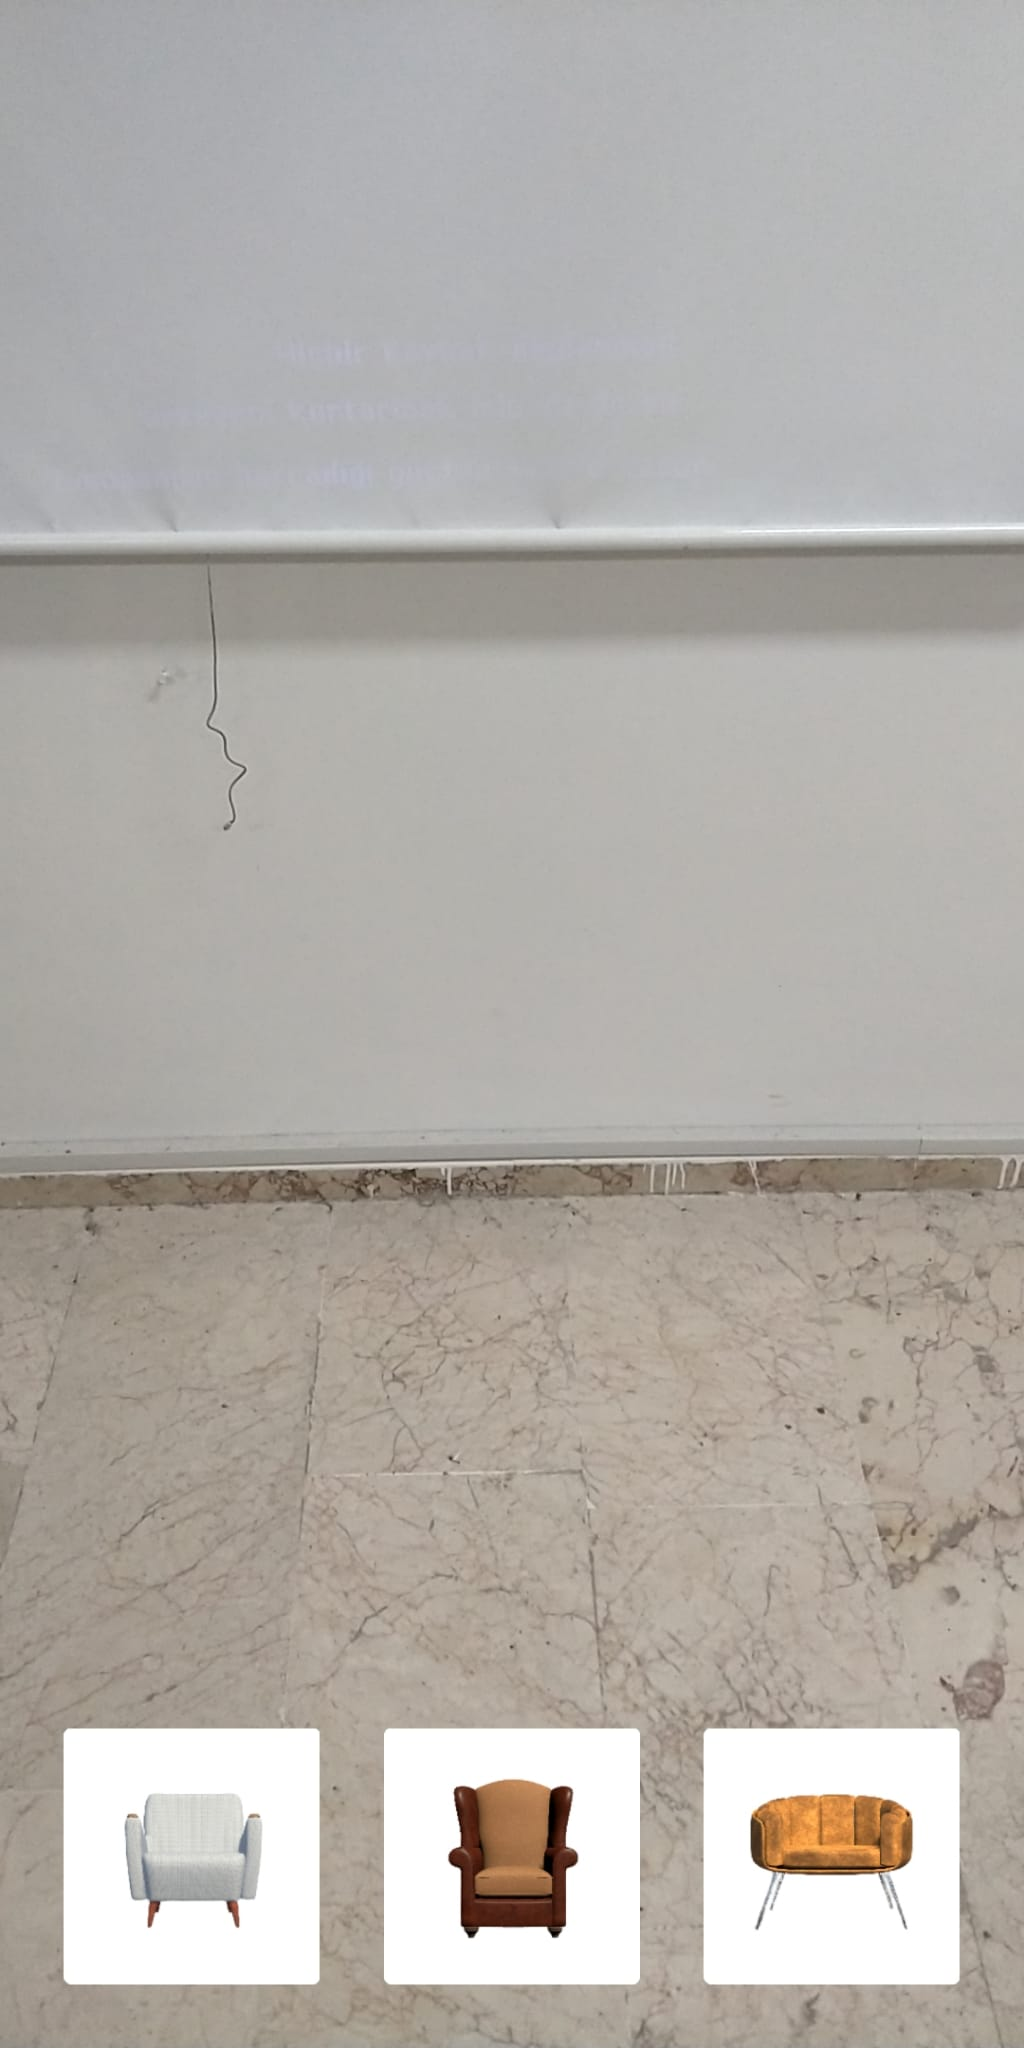
\includegraphics[width=.7\linewidth]{koltuk.jpeg}
			\caption{}\label{Fig:Data1}
		\end{minipage}\hfill
		\begin{minipage}{0.48\textwidth}
			\centering
			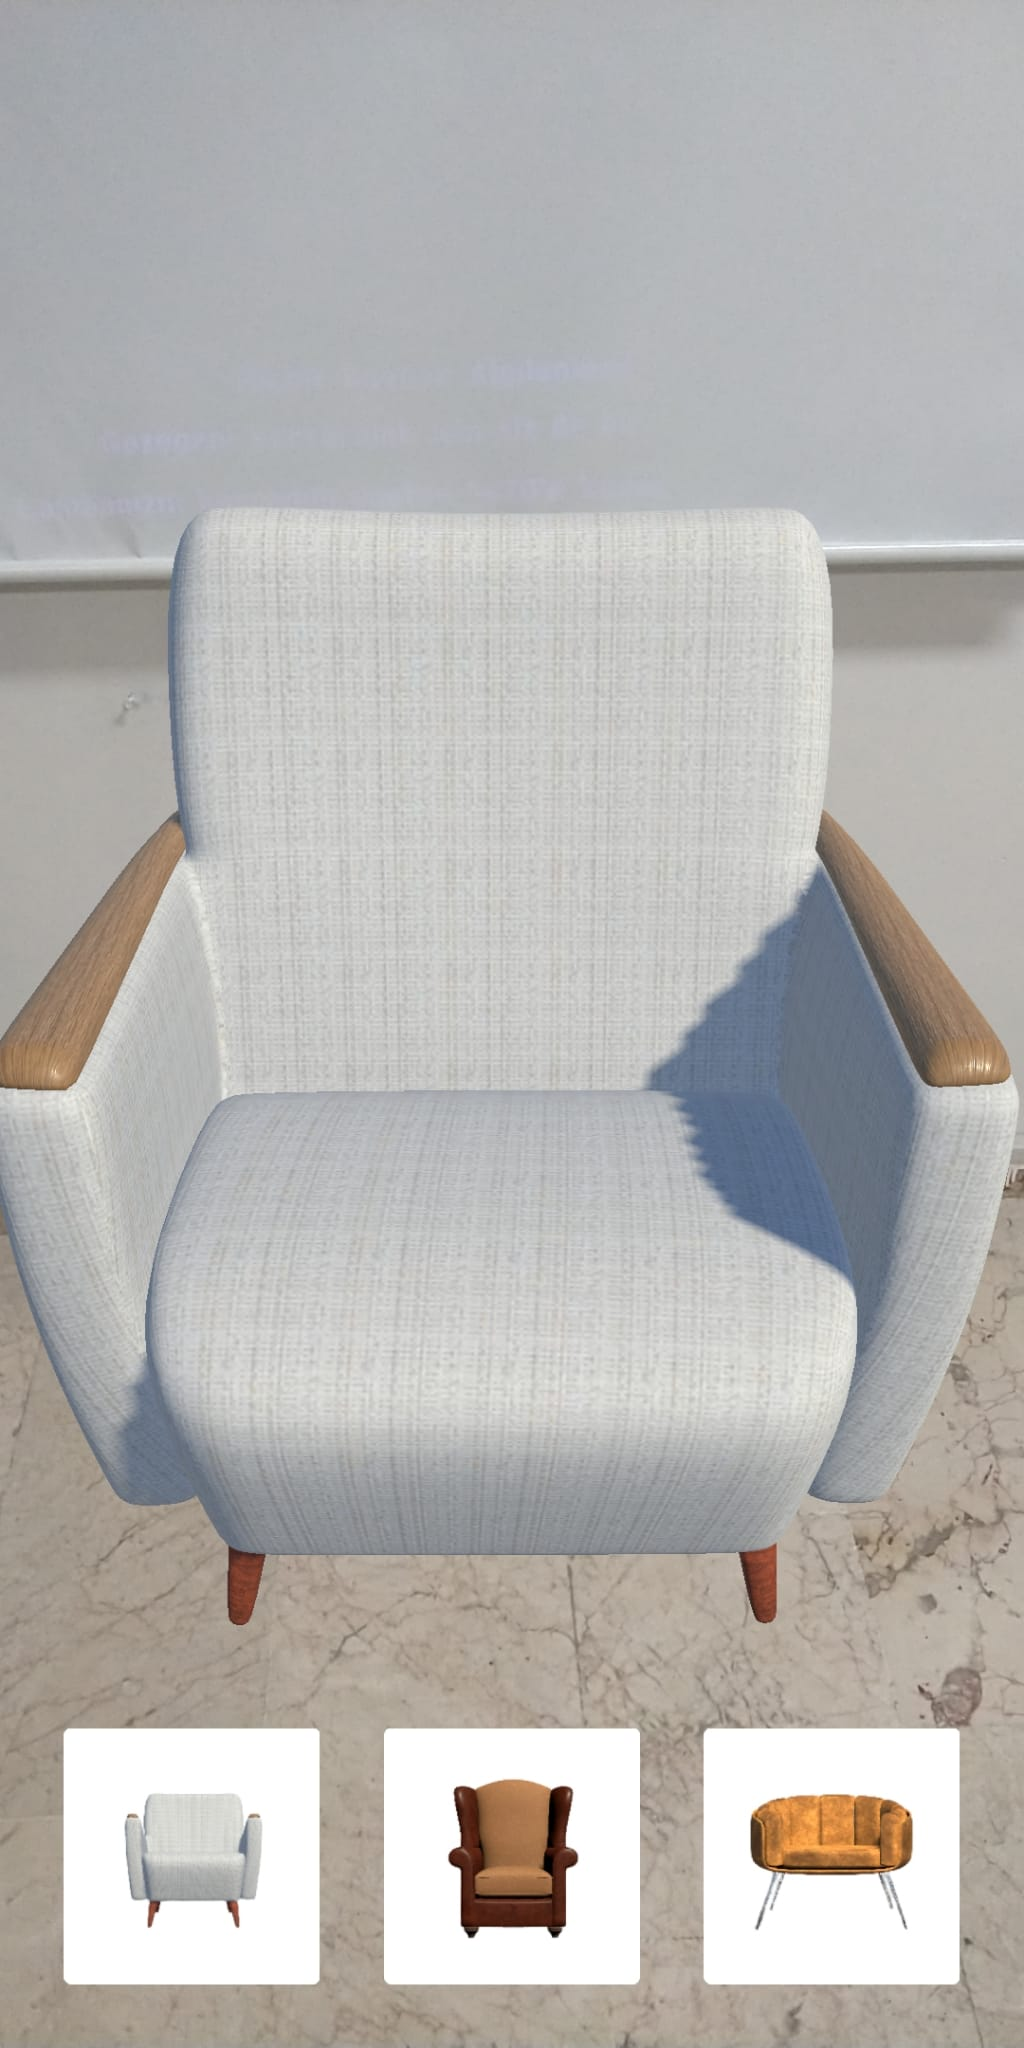
\includegraphics[width=.7\linewidth]{koltuk2.jpeg}
			\caption{}\label{Fig:Data2}
		\end{minipage}
	\end{figure}
	\newpage
		\title{Nuitrack Raporu Hafta 3}
	\author{Hasan Tekin}
	\date{\today}
	\maketitle
	
	\title{}
	\author{}
	\date{}
	\maketitle
		\setcounter{section}{0}
	
	\section{Nuitrack Nedir?}
	\begin{enumerate}
		\item Nuitrack, 3DiVi Inc. tarafından geliştirilen bir 3D izleme ara yazılımıdır. Bu, Android, Windows ve Linux'ta Doğal Kullanıcı Arayüzü (NUI) yeteneklerini sağlayan iskelet izleme ve hareket tanıma için bir çözümdür.
		
		Nuitrack çerçevesi çok dilli ve çapraz platformludur. Nuitrack API'leri, Doğal Etkileşimi kullanan uygulamalar geliştirmek için bir dizi arayüz içerir. Nuitrack'in temel amacı 3D sensörlerle iletişim için bir API oluşturmaktır.
		
		Nuitrack modülü ARM tabanlı işlemciler için optimize edilmiştir, bu da onu Android cihazlar ve gömülü platformlarla kullanabileceğiniz anlamına gelir.\cite{3DiVi}	
		
		
		
	\end{enumerate}
	\newpage
	
	\section{Temel Özellikleri}
	\begin{enumerate}
		
		\item Tüm Vücut İskelet Takibi (19 Eklem)
		\begin{figure}[!ht]
			\caption{}
			\centering
			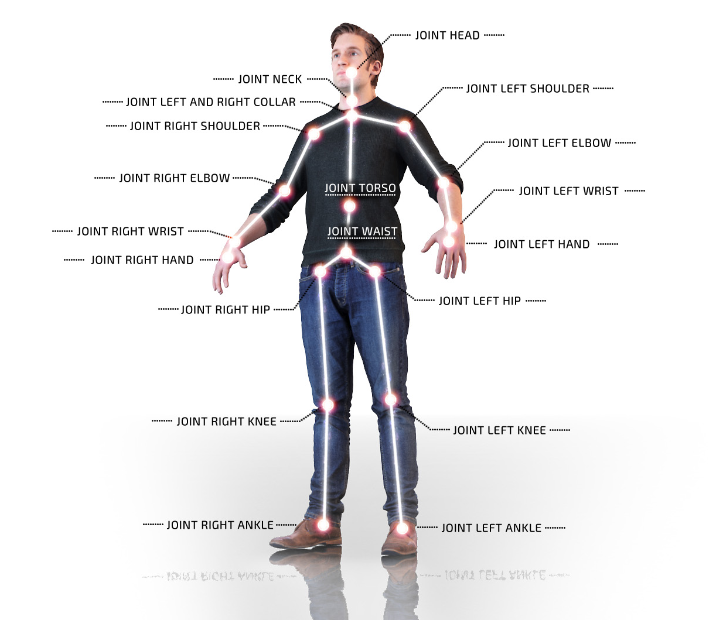
\includegraphics[width=0.8\textwidth]{Nuitrack.PNG}
			
			\label{dino1}
			Şekil \ref{dino1} de 19 eklem gösterilmiştir.\cite{3DiVi}	
		\end{figure}
		\newpage
		\item 3D Nokta Bulutu
		\begin{figure}[!ht]
			\caption{}
			\centering
			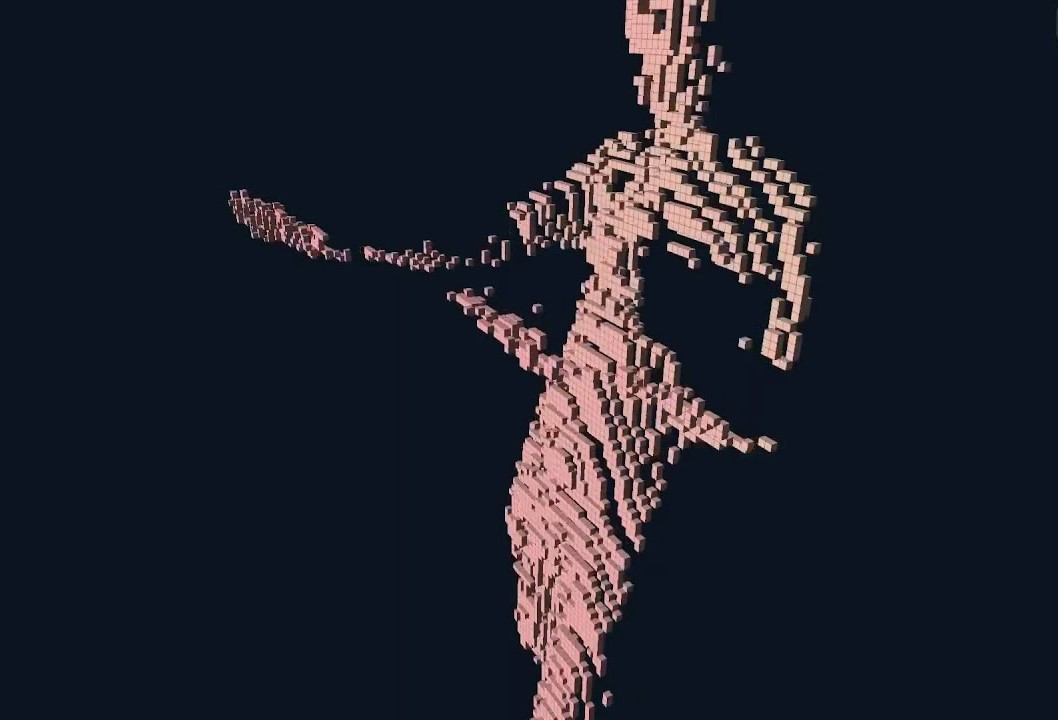
\includegraphics[width=0.8\textwidth]{Nuitrack1.jpg}
			
			\label{dino}
			Şekil \ref{dino1} de 3D nokta bulutu gösterilmiştir.\cite{3dPointCloud}	
		\end{figure}
		\item Kullanıcı Maskeleri
		\item Hareket Tanıma
		\item Android, Windows ve Linux için platformlar arası SDK
		\item 3D Sensör bağımsız Unity ve Unreal Engine Eklentileri
		\item OpenNI 1.5 uyumludur: OpenNI modülü, Kinect ve Asus Xtion için geliştirilen OpenNI tabanlı uygulamalarınızı Android dahil diğer platformlara taşımanıza olanak tanır.
		
	\end{enumerate}
	
	
	
	
	\section{Uygulama Alanları}
	\begin{enumerate}
		\item Windows/Linux/Android için Doğal Kullanıcı Arayüzü (NUI)
		\item Oyunlar ve Eğitim (Fitness, Dans Dersleri)
		\item Tıbbi Rehabilitasyon
		\item Akıllı Ev
		\item AR / VR için Tam Vücut Takibi
		\item Kitle Analitiği
		\item Robot Görüşü
		
		\cite{3DiViBasic}
		
	\end{enumerate}
	
	\section{Aldığım Hatalar}
	\begin{figure}[!ht]
		\caption{}
		\centering
		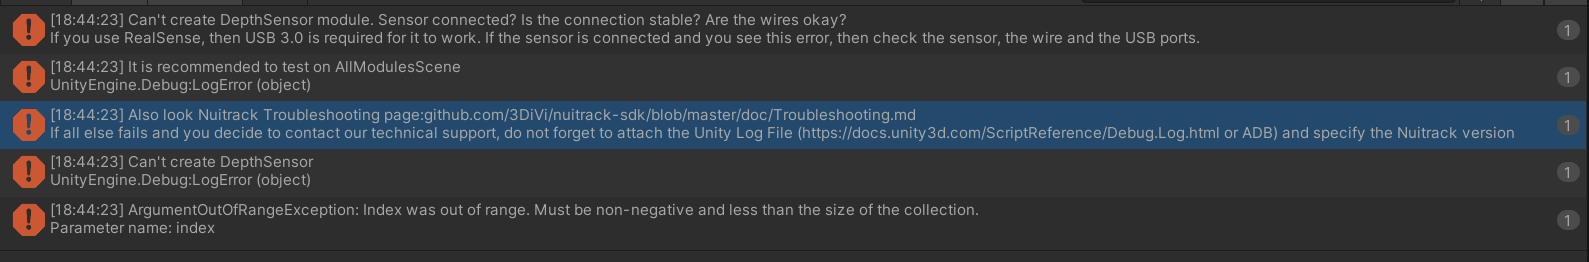
\includegraphics[width=0.8\textwidth]{unityHataPNG.PNG}
		
		\label{Hata}
		
	\end{figure}
	
	\newpage
	
	\title{Artırılmış Gerçeklik Raporu Hafta 4}
	\author{Hasan Tekin}
	\date{\today}
	\maketitle
	\setcounter{section}{0}
	
	
	\section{AR Foundation }
	\begin{enumerate}
		\item Artırılmış gerçeklik (AR) günümüz yazılım endüstrisinde en hızlı büyüyen teknolojilerden biridir. Birçok uygulama makyaj, kamera filtreleri ve sahne efektlerini simüle etmek için AR teknolojisini kullanmaktadır.
		
		Sıfırdan bir AR uygulaması geliştirmek kolay bir iş değildir. Görüntüleme işleme, hareket izleme, uzamsal analiz ve hatta makine öğrenimi için gelişmiş algoritmaları bilmeniz gerekir. Neyse ki Apple ve Android, işi kolaylaştırmak için gerekli algoritmaları düzenli paketler halinde bir araya getiren kendi AR yazılım geliştirme kitlerini (SDK'lar) geliştirdi.
		
		Ne yazık ki, hem iOS hem de Android cihazlar için bir AR uygulaması oluşturmak istiyorsanız, her iki SDK'yı da kullanmanız gerekir, bu da geliştirme çabalarınızı iki katına çıkarır. Bunu çözmek için Unity, AR Foundation adında kullanışlı bir kütüphaneye sahiptir. Bu kütüphane, tek bir kod tabanı ile hem iOS hem de Android için AR uygulamanızı oluşturmanıza yardımcı olabilir!\cite{ARFoundation}
		
	\end{enumerate}
	\newpage
	\begin{figure}[!ht]
		\caption{}
		\centering
		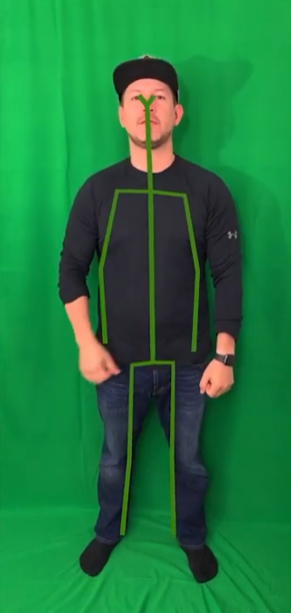
\includegraphics[height=0.8\textheight]{ARFoundation.PNG}
		
		\label{ARFoundation}
	\end{figure}
	Şekil \ref{ARFoundation} de gösterilen bu resim ARFoundation kullanılarak Gerçek Zamanlı Vücut İskeleti Oluşturmak için Vücut Takibi yapar.\cite{Youtube}
	
	
	
	
	
	\newpage
	
	
	\title{}
	\author{}
	\date{}
	\maketitle
	% Section değerini sıfırlıyor alt başlık değerini
	\setcounter{section}{0}
	
	\section{MediaPipe Nedir ?}
	\begin{enumerate}
		\item MediaPipe, Google tarafından geliştirilen bir açık kaynaklı bir kütüphanedir ve görüntü ve video işleme için kullanılır. Temelde, işaret işleme, nesne algılama, yüz tanıma, el izleme, vücut izleme gibi işlemlerde kullanılır.
	\end{enumerate}
	\begin{figure}[!ht]
		\caption{}
		\centering
		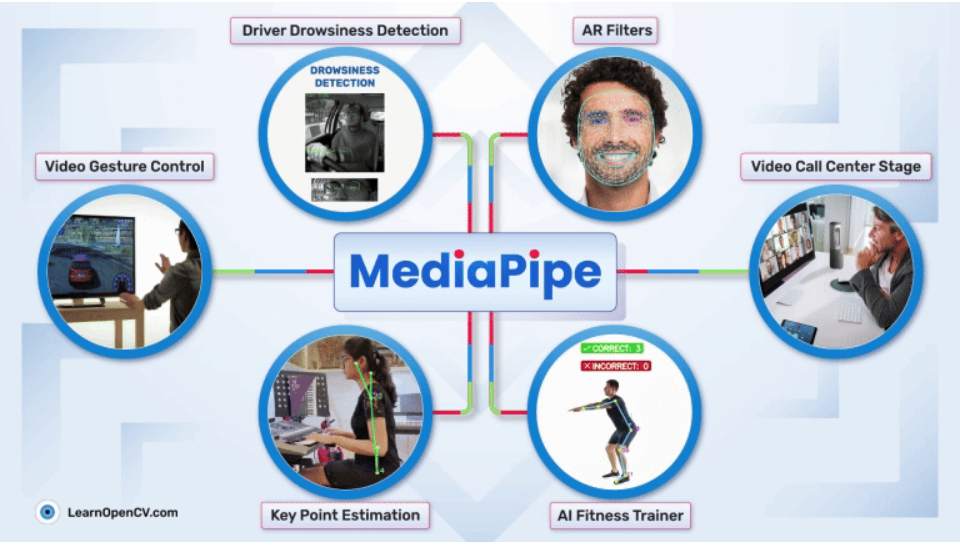
\includegraphics[width=0.8\textwidth]{mediaPipe.PNG}
		
		\label{mediaPipe}
	\end{figure}
	Şekil \ref{mediaPipe} de gösterilen bu görsel mediaPipe'ın kullanım alanlarını göstermektedir.\cite{MediaPipe}
	\newpage
	\section{MediaPipe Hareket Takibi Örneği}
	\begin{enumerate}
		\item Bu örneğin temel amacı, Unity ve MediaPipe kullanarak basit seviyede bir hareket takibi sistemi geliştirmektir. Bu örnekteki amaç bir kişinin hareketlerini gerçek zamanlı olarak izlemeyi hedeflemektedir. MediaPipe kullanılarak kameradan gelen görüntü işlenecek ve izlenen kişinin vücudundaki eklemler tanımlanarak hareketleri takip edilecektir.
		
	\end{enumerate}
	
	\begin{figure}[!ht]
		\caption{}
		\centering
		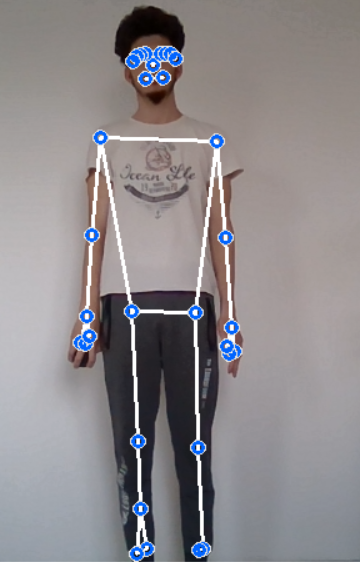
\includegraphics[height=0.8\textheight]{Ben2.png}
		
		\label{Ben}
	\end{figure}
	\newpage
	Şekil \ref{Ben} de gösterilen bu görselde eklemler gösterilmektedir.
	\begin{figure}[!ht]
		\caption{}
		\centering
		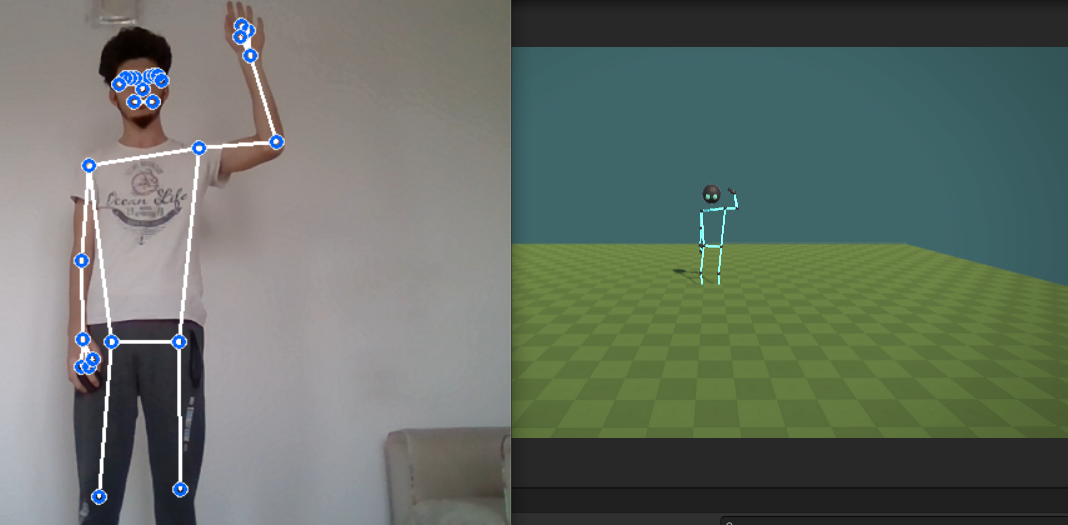
\includegraphics[width=0.8\textwidth]{Klon.PNG}
		
		\label{Klon}
	\end{figure}
	\newpage
	Şekil \ref{Klon} de gösterilen bu görselde gerçek zamanlı hareket gösterilmektedir.
	\newpage
	
	
	%Kaynakçayı yazdırmak
	\bibliographystyle{ieeetr}
	\bibliography{references.bib} 
	%\printbibliography %Prints bibliography
	
	
\end{document}